
%%%%%%%%%%%%%%%%%%%%%%%%%%%%%%%%%%%%%%%%%%%%%%%%%%%%%%%%%%
\chapter{Conclusions and Future Work}
\label{chapter_conclusions_and_future_work}
%%%%%%%%%%%%%%%%%%%%%%%%%%%%%%%%%%%%%%%%%%%%%%%%%%%%%%%%%%

\section{Conclusions}

\newtext
{
We presented three deformation-driven packing methods.
FLOWPAK is a method to deform and pack long thin elements to follow a vector field.
RepulsionPak is a method that uses repulsion forces to pack and deform
elements that are represented as mass-spring systems.
AnimationPak is an extension of RepulsionPak that packs animated 2D elements,
each an extruded 3D shape in a spacetime domain.
}

\newtext
{
Given a small element library, 
we demonstrated that deformation-driven methods can create element compatibilities
and fill the container effectively.
Repeated elements give a sense of uniformity but deformation creates a sense of variety.
%As element compatibilities are increased, the negative space is more even.
}

\newtext
{We discussed the evenness of negative space as an indicator of the quality of a packing.
We measured the evenness using three statistical metrics:
spherical contact probabilities, histograms of distance transforms, and overlap functions.
}

\section{Future Work}

\newtext
{
This thesis \nnewtext{is} only the tip of the iceberg of packing research \newtext{and}
we see many possibilities for future work.
}

%%%%%%%%%%%%%%%%%%%%%%%%%%%%%%%%%%%%%%%%%%%%%%%%%%%%%%%%%%%%%%%%%%%%%%%%%%%%%%%%%%%%%%%%%%
%%%%%%%%%%%%%%%%%%%%%%%%%%%%%%%%%%%%%%%%%%%%%%%%%%%%%%%%%%%%%%%%%%%%%%%%%%%%%%%%%%%%%%%%%%
%%%%%%%%%%%%%%%%%%%%%%%%%%%%%%%%%%%%%%%%%%%%%%%%%%%%%%%%%%%%%%%%%%%%%%%%%%%%%%%%%%%%%%%%%%
\subsection{Spacious Element Arrangements}

\nnewtext{We would like to create element arrangements with varying negative space widths,
some are wide enough to generate spacious element arrangements.
Evenness of negative space is only one of many design considerations to create aesthetically pleasing element packings.
As discussed in Chapter~\ref{chapter_introduction}, variations in the balance of positive and negative space can be used to emphasize focal points.
It would be interesting to incorporate a density field, similar to stippling artwork by Secord~\cite{Secord2002}.
In a low density area, elements are smaller and negative space is wider. 
Conversely, a high density area can be represented by bigger elements and narrower negative space. 
It would also be great to use a bitmap image as a container, 
we then perform image segmentation algorithm to produce subregions, each has a different element density.
}


% aesthetic arrangement

% texture synthesis
\nnewtext{
Another potential extension to our deformation-driven methods is synthesizing discrete texture,
where element distributions are more important than element interlocking.
Because of the generous negative space, we can run RepulsionPak simulation without the growth process.
However, the main challenge is to incorporate inter-element spatial relationships from an exemplar to the RepulsionPak simulation.
Lastly, generating a pleasing arrangement from a fully automated method is difficult, 
so it also would be interesting to incorporate an interactive tool by Reinert et al.~\cite{Reinert2013} 
that can infer an artist's intention to generate an artistic arrangement.
}
%However, the main challenge is to mimic the element distribution in an exemplar.
%We would like to investigate whether the technique developed by Ijiri et al.~\cite{Ijiri2008a} can be incorporated to RepulsionPak.
%Ijiri et al. encoded inter-element spatial relationships by triangulating the element positions.
%The edges of the triangle mesh can be included to RepulsionPak simulation as edge springs.  



%%%%%%%%%%%%%%%%%%%%%%%%%%%%%%%%%%%%%%%%%%%%%%%%%%%%%%%%%%%%%%%%%%%%%%%%%%%%%%%%%%%%%%%%%%
%%%%%%%%%%%%%%%%%%%%%%%%%%%%%%%%%%%%%%%%%%%%%%%%%%%%%%%%%%%%%%%%%%%%%%%%%%%%%%%%%%%%%%%%%%
%%%%%%%%%%%%%%%%%%%%%%%%%%%%%%%%%%%%%%%%%%%%%%%%%%%%%%%%%%%%%%%%%%%%%%%%%%%%%%%%%%%%%%%%%%
\subsection{Element Construction}

\deadtext{Good element shapes are difficult to design.} 
\nnewtext{We would like to explore techniques to assist users in constructing element shapes.}
A simple example can be seen in a FLOWPAK packing, 
where we allow the user to construct additional motifs automatically 
by tracing the shapes of pockets of negative space (Figure~\ref{result_bear_offset}). 


\newtext{Earlier data-driven packing techniques achieve variety 
by assembling a large library of element shapes. 
In FLOWPAK and RepulsionPak, we used deformation to amplify the variety of a much smaller element library. 
Other approaches may allow us to generate variety in different ways. 
For example, we could construct \textit{modular} elements by assembling them from smaller subparts (Figure~\ref{modular_element}). 
Past research has explored example-based and part-based assembly of modular objects~\cite{Baxter2006, Risser2010, Kalogerakis2012, Hurtut2012},
but more work is needed to make these tools practical and useful in the context of packings. 
Modularity is itself a kind of discrete mode of deformation, 
and we could mix-and-match parts during packing to improve packing quality. 
When fitting elements to the container boundary (Section~\ref{repulsionpak_shape_matching}) 
we could begin by choosing subparts that optimize the fit, and then build elements that contain those subparts.
Of course, compatibility could be further improved by deforming modular elements using the techniques in this thesis.}

\newtext{In the context of FLOWPAK, we are interested in exploring a simpler form of modularity, 
in which short subparts are assembled into larger shapes by threading them along curves, as illustrated in Figure~\ref{thread_branch}a.  
This approach to modularity might adapt itself particularly well to floral ornamentation.  
In that case, it would be natural to explore extensions to FLOWPAK that support branching structures instead of isolated curves, 
as in Figure~\ref{thread_branch}b.  
A challenge here is to identify pairs of subparts, and points on them, that support high-quality attachments. 
This quality can be measured geometrically, possibly aided by new algorithms for content-aware blending of vector shapes.  
It also has a semantic component; for example, a leaf shape can be attached to a stem, but not directly to a twig. 
Past research on ornament synthesis, such as DecoBrush~\cite{Lu2014} may be relevant here.}


\nnewtext{
Lastly, we would like to investigate a way to identify salient shapes in a source photograph to construct fixed elements.
We first perform an image segmentation algorithm~\cite{Comaniciu2002, Achanta2012} and the artist can select regions they think are important.
Each region is then vectorized to create a new fixed element.
Another approach is to replace these salient regions with highly deformed elements, 
similar to the calligraphy packing approaches~\cite{Xu2007, Zou2016}.
}

\begin{comment}
\nnewtext{Unlike data-driven methods and deformation-driven methods,
we would like to manufacture a new element on the fly during the packing process.
A simple example is demonstrated in a FLOWPAK result (Figure~\ref{result_bear_offset}), 
where new elements are created from the unused negative space.
A manufactured element is also useful to create a fixed element (Chapter~\ref{chapter_flowpak}),
which }can be done by discovering them as salient regions 
in source photographs, and extracting and vectorizing them.  This 
extraction must be carried out carefully, yielding enough fixed elements
to communicate a container clearly without disrupting the uniformity of
the design.

\nnewtext{Another idea is to manufacture \textit{modular} elements assembled from smaller subparts.
A modular element can increase its compatibility by swapping its subparts.
We would like to investigate several shape synthesis methods by 
Baxter and Anjyo~\cite{Baxter2006},
Risser et al.~\cite{Risser2010}, Kalogerakis et al.~\cite{Kalogerakis2012}, 
and Hurtut and Landes~\cite{Hurtut2012}. 
Data-driven methods can benefit from this approach as we are able to 
generate large combinations of elements from a collection of subparts.
We can also work toward uniformity amidst variety principle 
as we can generate similar elements with varying subparts.
}
\end{comment}

\begin{figure}
\centering
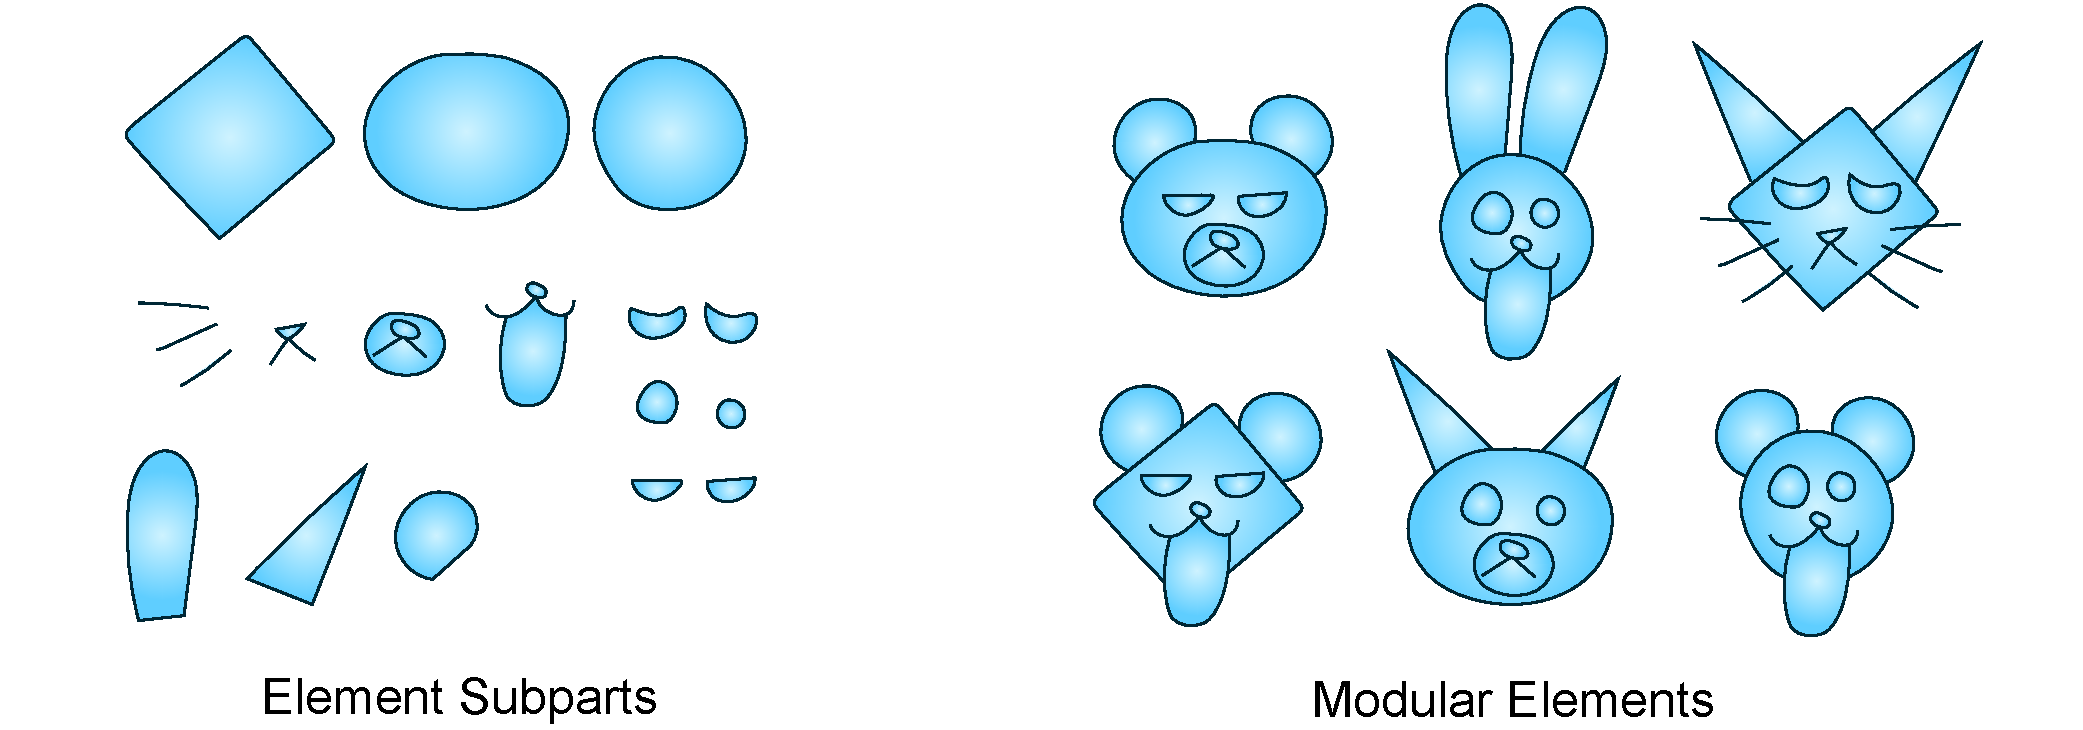
\includegraphics[width=1.0\textwidth]{figures/conclusions/modular.pdf}
\caption[Modular elements]
{ \label{modular_element} 
\newtext
{
Examples \newtext{of} modular elements assembled from smaller parts.
}
}
\end{figure}

\begin{comment}
\nnewtext{We also consider an idea of plant-style modular elements.
In Figure~\ref{thread_branch}a, we can
combine multiple shorter elements
by threading them on a curve to create a longer modular element.
In Figure~\ref{thread_branch}b, we can also
try to generate branching structures to resemble floral ornaments.
In both instances, there are several challenges we have to face.
First, we need a way to connect the overlapping segments of the elements together
to create smooth and plausible transitions.
An ornament synthesis method such as DecoBrush~\cite{Lu2014} may be worth investigating.
This leads us to a deeper research topic:
how to develop a content-aware blending method on vector graphics patterns.
Second, we also should consider the semantics of the element shapes.
Not every part of an element can be connected; for example, a twig
cannot be attached onto the tip of a leaf.}

\nnewtext{
Modular elements give us opportunities to perform a smarter element placement.
The first idea is similar to JIM method,
but we are able to backtrack to previous arrangements 
that not only have different element configurations but also
different part configurations.
The second idea is to perform partial shape matching only between salient container features and
element subparts. Once a matching subpart is attached to a salient feature, we can then manufacture an entire
element based on that subpart.}
\end{comment}




\begin{figure}
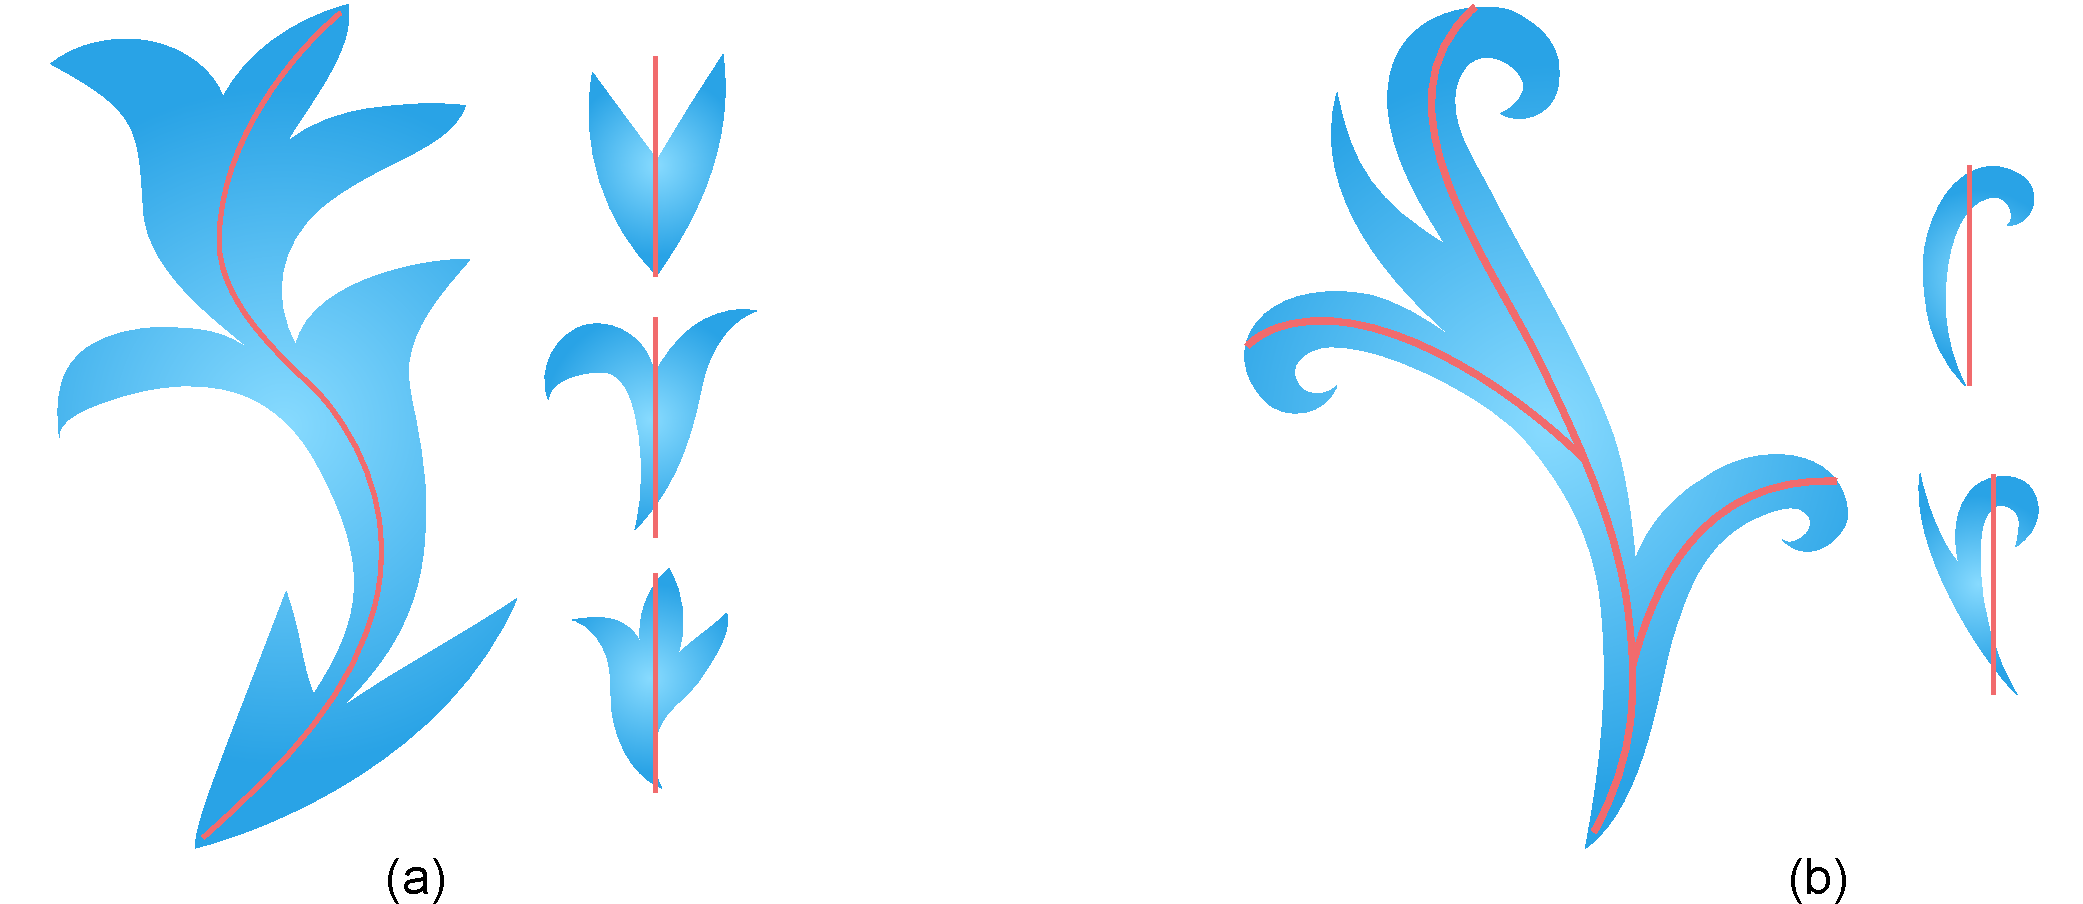
\includegraphics[width=1.0\textwidth]{figures/conclusions/thread_branch_3.pdf}
\caption[Element threading and branching]
{ \label{thread_branch} 
\newtext
{
Plant-style modular elements.
(a) \newtext{A larger element is constructed by threading multiple subparts along a curve.}
(b) \newtext{Multiple streamlines are joined in a branching structure.}
}
}
\end{figure}





%%%%%%%%%%%%%%%%%%%%%%%%%%%%%%%%%%%%%%%%%%%%%%%%%%%%%%%%%%%%%%%%%%%%%%%%%%%%%%%%%%%%%%%%%%
%%%%%%%%%%%%%%%%%%%%%%%%%%%%%%%%%%%%%%%%%%%%%%%%%%%%%%%%%%%%%%%%%%%%%%%%%%%%%%%%%%%%%%%%%%
%%%%%%%%%%%%%%%%%%%%%%%%%%%%%%%%%%%%%%%%%%%%%%%%%%%%%%%%%%%%%%%%%%%%%%%%%%%%%%%%%%%%%%%%%%
\subsection{Beyond 2D}

\nnewtext{Inspired by the 3D shaded skull packing in Figure~\ref{paul_daichi_packings},}
\nnewtext{we would like to explore the use of deformation-driven methods to create packings on surfaces.}
\nnewtext{It should be possible to adapt FLOWPAK and RepulsionPak to pack elements on 3D 
surfaces by computing geodesic distances to generate physical forces.}
\nnewtext{Packings on surfaces are also useful in a fabrication context, for example, 
creating printed objects in the style of previous work like that of Chen et al.~\cite{Chen2017}.}
We could exploit boundary compatibilities to discover ideal locations to connect neighbouring elements.
Alternatively, it would be interesting to 3D print the 
negative space, which is already connected due to the absence of overlaps.
The resulting packing \newtext{would be more like a filigree~\cite{Chen2016}, 
with thin wires bounding holes in the shapes of the elements.}

\newtext{Many of the techniques in this thesis could be adapted
to develop a deformation-driven method for packing purely spatial
3D objects in a 3D container.  
We would like to evaluate the
expressivity and visual quality of deformation-driven 3D packings 
in comparison to other 3D packing techniques.
One potential issue is that elements in the middle \newtext{of the container} may be fully occluded by their neighbours,
which would render them useless as they cannot be viewed.
This problem will arise especially in a dense 3D packing of small elements.}

\begin{comment}
\nnewtext{Another interesting idea would be generating a bas-reliefs using a packing method,
which can be called as a 2.5D packing.
Figure~\ref{borobudur} shows a two bas-reliefs from Borobudur temple in Indonesia,
each relief consists of tight arrangement of human shapes although it does not 
have interlocking style of packings.
We see this problem as arranging non-overlapping 3D elements on surfaces, 
which include not only 2D panels but also any 3D surfaces.
Each 3D element can still rotate in all three axes but still attached to the surface.
As seen in the Borobudur reliefs, elements may occlude but they do not actually overlap.
It would be interesting to investigate aesthetics value of 2.5D packings that allow some amount of occlusions
as the consequence of 3D rotations but are still overlaps free.
}
\end{comment}

\newtext{
It may also be possible to construct interesting packings of 3D objects constrained to lie near a surface.
Figure~\ref{borobudur} shows two stone bas-reliefs from the Borobudur temple on the island of Java. 
Each relief consists of a tight, albeit non-interlocking, arrangement of human shapes. 
We are interested in constructing similar arrangements using deformation-driven packing, 
with elements that are required to lie on a shared surface. 
The interactions between elements during the packing process 
may cause them to occlude each other but without interpenetration. 
We are curious to know how occlusions affect aesthetics in the context of bas-reliefs like these.
}


\begin{figure}
\centering
\includegraphics[width=1.0\textwidth]{figures/conclusions/borobudur.pdf}
\caption[Element arrangements in bas-reliefs]
{ \label{borobudur} 
\newtext
{
Bas-reliefs from Borobudur temple. These
bas-reliefs give us an idea to generate a packing of 3D objects on \newtext{a surface}.
Individual element can still rotate in 3D to align itself with its neighbours.
The photographer of the left image was Michael Gunther, and the right image was taken by Michel Estermann.
}
}
\end{figure}

%%%%%%%%%%%%%%%%%%%%%%%%%%%%%%%%%%%%%%%%%%%%%%%%%%%%%%%%%%%%%%%%%%%%%%%%%%%%%%%%%%%%%%%%%%
%%%%%%%%%%%%%%%%%%%%%%%%%%%%%%%%%%%%%%%%%%%%%%%%%%%%%%%%%%%%%%%%%%%%%%%%%%%%%%%%%%%%%%%%%%
%%%%%%%%%%%%%%%%%%%%%%%%%%%%%%%%%%%%%%%%%%%%%%%%%%%%%%%%%%%%%%%%%%%%%%%%%%%%%%%%%%%%%%%%%%
\subsection{Collaborations with Artists}


%We are confident that our methods can 

\newtext{
Collaborations with artists can provide us invaluable feedback for our deformation-driven methods.
Two artists have used RepulsionPak to generate packings in Figure~\ref{paul_daichi_packings},
although we did not \newtext{collect formal feedback or data on their experiences}.
\newtext{After RepulsionPak was demonstrated at a large public event, we also received expressions of interest and enthusiasm from online graphic design communities.}}

%We also receive interests from online communities to use RepulsionPak for graphic design applications.
%We also demoed RepulsionPak at a conference and we received interests from online communities to release RepulsionPak as a software product.
%We also demoed RepulsionPak at a conference and we received interests from online communities to make RepulsionPak be available as

\newtext{We would like to develop} an interactive user \newtext{interface} for our packing methods.
Examples of recent work in this style include research
by Zehnder et al.~\cite{Zehnder2016}, Gieseke et al.~\cite{Gieseke2017}, 
and Hsu et al.~\cite{Hsu2020}, which let the user directly place and manipulate
elements while a composition is being created.
\newtext{
Inspired by doodle murals by Joe Whale (Figure~\ref{doodle_boy}), 
it would be interesting \newtext{to develop an interactive installation in which users could interact with a live packing on a large touch-screen display}.
}

\nnewtext
{
It would also be interesting to create a system to assist an artist for creating arrangements from physical elements
by using a camera-equipped augmented reality headset. The camera is used to scan these elements which are then processed by the system.
Finally, the headset displays a suggestion of an element arrangement which the artist can follow.
}

\newtext{In the context of animated packings,} 
we were only able to find a single example from The Simpsons (Figure~\ref{fig_animationpak_lisa_packing}). 
\newtext{We believe these designs are rare because they have been so difficult to create using conventional software.}
\newtext{We} would like to engage with artists to understand the aesthetic value and limitations
of AnimationPak.

\begin{figure}
\centering
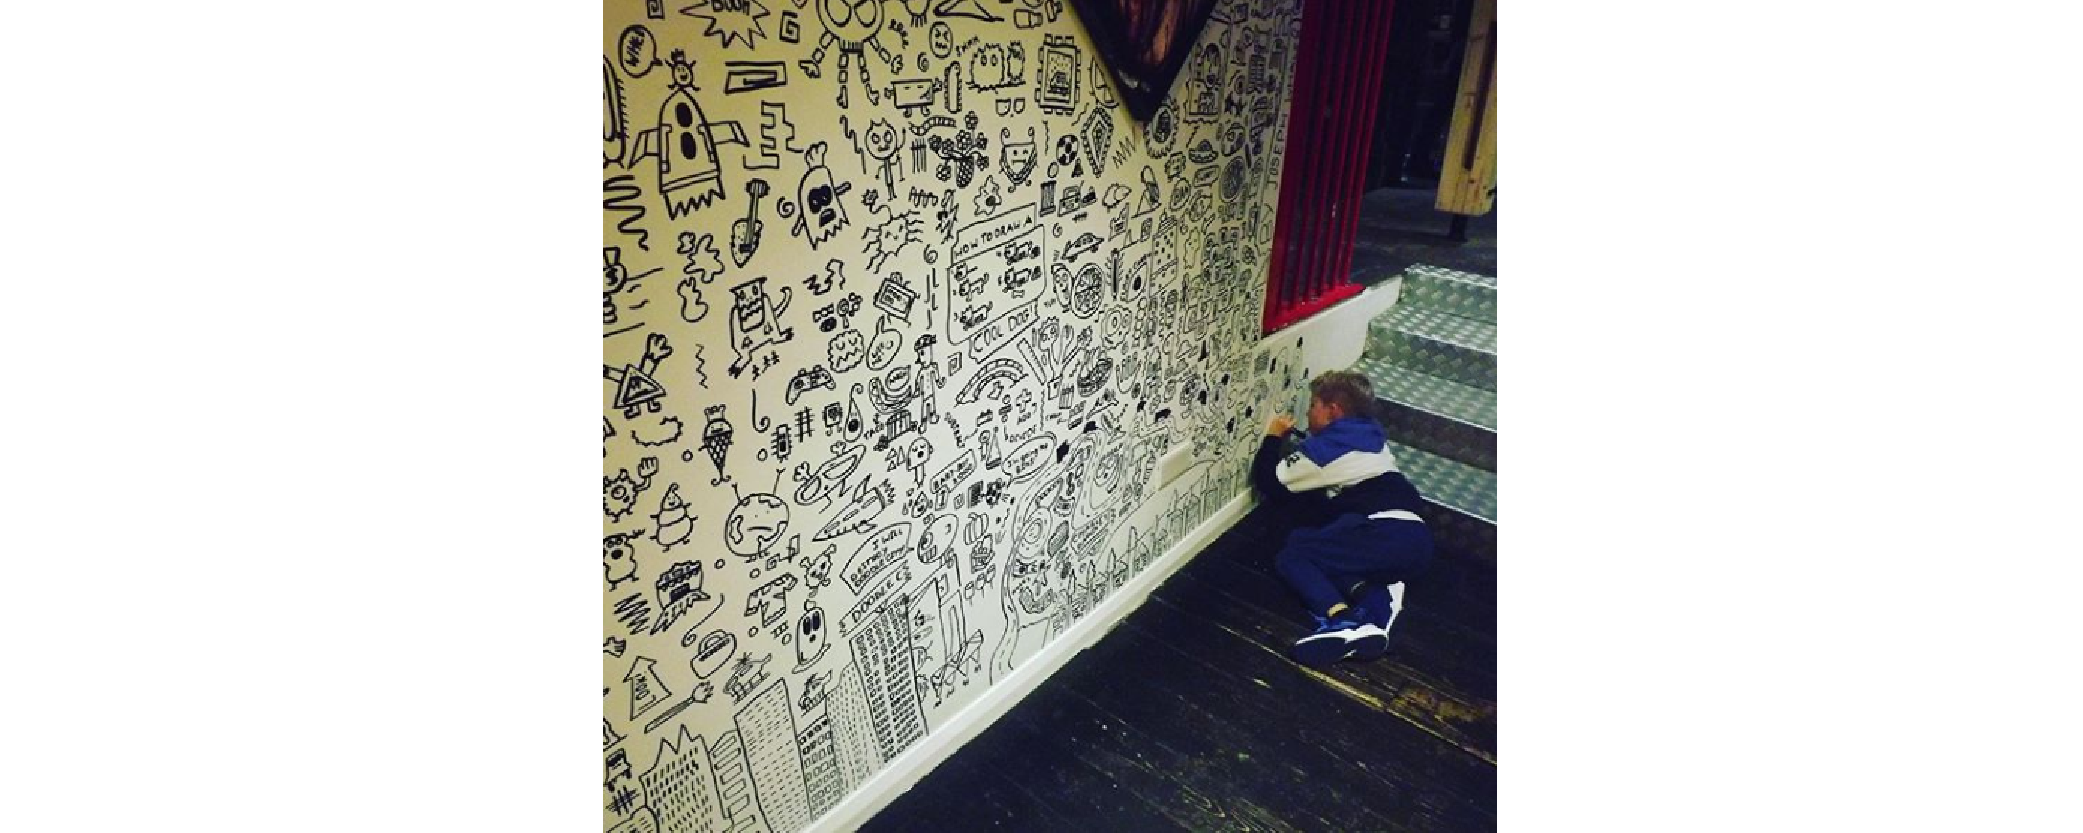
\includegraphics[width=1.0\textwidth]{figures/conclusions/doodle_boy.pdf}
\caption[A doodle mural by Joe Whale]
{ \label{doodle_boy} 
\newtext
{
A young artist, Joe Whale, is drawing a doodle mural. 
The photograph is taken from instagram.com/thedoodleboy.co.uk.
}
}
\end{figure}

%%%%%%%%%%%%%%%%%%%%%%%%%%%%%%%%%%%%%%%%%%%%%%%%%%%%%%%%%%%%%%%%%%%%%%%%%%%%%%%%%%%%%%%%%%
%%%%%%%%%%%%%%%%%%%%%%%%%%%%%%%%%%%%%%%%%%%%%%%%%%%%%%%%%%%%%%%%%%%%%%%%%%%%%%%%%%%%%%%%%%
%%%%%%%%%%%%%%%%%%%%%%%%%%%%%%%%%%%%%%%%%%%%%%%%%%%%%%%%%%%%%%%%%%%%%%%%%%%%%%%%%%%%%%%%%%
\subsection{Packing Evaluation}

We would like to develop \newtext{other quantitative metrics} to evaluate
how well an ornamental design fulfills other design principles.
\newtext{In Chapter~\ref{chapter_flowpak}, we argue that visual flow and
``uniformity amidst variety'' are important in attractive packings.} 
In another study, Wong et al.~\cite{Wong1998} describe basic design
principles for decorative arts: repetition, balance, and conformation
to geometric constraints. 

\newtext{\newtext{Currently, we measure only the evenness of negative space.}
A measure of element deformation in a composition would permit 
a comparison against future deformation-driven techniques.
In RepulsionPak, we can measure \newtext{a packing's} potential energy at equilibrium.
However, there are some questions to answer.
Can we measure how deformations are perceived? How much they affect the aesthetics of packings?
Such measurements could help us develop better deformation algorithms in general, not just in the context of packings.}

All three metrics described in Chapter~\ref{chapter_qualitative_metrics} are only for evaluating 2D packings.
While they extend naturally to three purely spatial dimensions, 
it is not clear whether they can be adapted to the spacetime context.  
We would like to investigate spatial statistics for the quality of animated packings created by AnimationPak.
%that correlate
%with human perceptual judgments.

\newtext{
More broadly, although our algorithms and measurements are derived from careful study of packings created by artists, there is no guarantee that a statistic like the evenness of negative space is a suitable proxy for human aesthetic judgment. Future work should seek to articulate mathematical criteria that correlate with qualitative packing quality, using perceptual studies on human subjects.}

